\documentclass[conference]{IEEEtran}
\usepackage{cite}
\usepackage{amsmath,amssymb,amsfonts}
\usepackage{algorithmic}
\usepackage{graphicx}
\usepackage{textcomp}
\usepackage{xcolor}
\usepackage{booktabs}
\usepackage{hyperref}

\hypersetup{
    colorlinks=true,
    linkcolor=blue,
    citecolor=blue,
    urlcolor=blue
}

\begin{document}

\title{A Rigorous Reality Check on Quantum-Enhanced Network Intrusion Detection: Empirical Benchmarking, Classical Surrogates, and Cross-Dataset Limits}

\author{
\IEEEauthorblockN{Khatwang Madhav Yippili}
\IEEEauthorblockA{\textit{Department of Mathematical Sciences and Computing} \\
\textit{Sri Sathya Sai Institute of Higher Learning}\\
Prasanthi Nilayam, Andhra Pradesh, India}
}

\maketitle

\begin{abstract}
Network intrusion detection systems (NIDS) deployed in modern Security Operations Centers (SOCs) face acute alert fatigue driven by high false alarm rates on bursty benign traffic. Under the Amaravati Quantum Valley (AQV) Use Case UC-029 mandate (\textit{Cybersecurity \& Quantum-Safe Infrastructure}), this paper presents an empirical, zero-trust benchmark of hybrid quantum-classical neural network architectures operating under a strict 4-qubit Noisy Intermediate-Scale Quantum (NISQ) hardware budget ($N \le 4$). Across seven paradigms on real UNSW-NB15 flow records, we conduct an expanded 30-seed hypothesis testing protocol ($N=30$) and demonstrate that the performance gap between Full VQC ($93.65\%$ accuracy) and Bypassed controls ($93.61\%$ accuracy) is statistically non-significant ($p = 0.6266$, Cohen's $d = 0.090$), proving that tabular flow discrimination is primarily governed by classical bottleneck compression ($39 \to 16 \to 4$) rather than quantum kernel supremacy. Crucially, we introduce parameter-matched Classical Random Fourier Feature (RFF) and Trainable Fourier surrogates to test if quantum expressivity transcends classical harmonic representations. In cross-dataset domain transfer from UNSW-NB15 to CIC-IDS2017 with strict per-model RNG isolation, Hybrid VQC ($48.22\% \pm 4.31\%$ F1, $54.85\%$ retention) is statistically indistinguishable from classical Fourier surrogates (RFF: $49.06\% \pm 13.71\%$ F1, $p = 0.9087$; Trainable Fourier: $49.20\% \pm 3.59\%$ F1, $p = 0.7910$), while classical Fourier models maintain a $77\times$ latency advantage ($0.066\text{ ms}$ vs $5.088\text{ ms}$). Furthermore, Matrix Inversion (M3) readout mitigation mathematically recovers $46.6\%$ of Pauli-$Z$ expectation drift under $3\%$ bit-flip noise ($p = 0.03$), with condition numbers remaining bounded ($\kappa(\mathbf{M}) \le 2.44$) even under $10\%$ noise. These findings establish that 4-qubit variational circuits act functionally as classical Fourier feature transforms without unique quantum representational supremacy on classical network flows.
\end{abstract}

\begin{IEEEkeywords}
Quantum Machine Learning, Network Intrusion Detection, Variational Quantum Circuits, NISQ, Readout Mitigation, UNSW-NB15, Model Ablation.
\end{IEEEkeywords}

\section{Introduction}
Modern enterprise and state-level Security Operations Centers (SOCs) monitor high-throughput network backbones where subtle zero-day intrusions, stealthy exfiltration, and reconnaissance probes overlap heavily with benign network telemetry in continuous statistical feature space. In practical SOC workflows, even a modest $1\%$ to $2\%$ increase in False Positive Rate (FPR) translates to thousands of false alerts per day, inducing severe analyst alert fatigue and increasing the mean-time-to-detect (MTTD) for critical breaches.

Under national quantum roadmap initiatives and the Amaravati Quantum Valley (AQV) Use Case UC-029 framework, Quantum Machine Learning (QML) has emerged as a promising paradigm for modelling complex network traffic distributions. By mapping classical flow features into high-dimensional Hilbert spaces ($\mathcal{H} = \mathbb{C}^{2^N}$) via parameterized quantum circuits (PQCs), quantum kernels have the theoretical potential to resolve non-linearly separable decision boundaries that confound classical linear readouts.

However, existing literature evaluating QML on network flow benchmarks often suffers from four severe methodological vulnerabilities:
\begin{enumerate}
    \item \textit{Data Leakage \& Shortcut Memorization:} Many studies report near-$100\%$ accuracy by inadvertently retaining unique row identifiers (\texttt{id}), protocol metadata, or by fitting normalization scalers across entire datasets rather than strictly on training splits.
    \item \textit{Unsubstantiated Quantum Advantage Claims:} Improvements in hybrid pipelines are frequently attributed to ``quantum supremacy'' without evaluating depth-matched classical controls or conducting ablation tests to isolate whether the quantum circuit or the surrounding classical neural layers drove classification gains.
    \item \textit{Idealized Hardware Assumptions:} Evaluations predominantly assume infinite-precision, noiseless statevector simulation without quantifying vulnerability to physical gate depolarizing and measurement readout errors.
    \item \textit{Absence of Latency Benchmarking:} Studies omit single-sample inference latency measurements, obscuring the severe state-preparation and circuit dispatch overheads that impede real-time packet-rate deployment.
\end{enumerate}

To address these vulnerabilities, this paper establishes a zero-trust, multi-paradigm empirical benchmark on real UNSW-NB15 flow data under a strict $N \le 4$ qubit budget. We systematically structure our analysis through three complementary perspectives:
\begin{itemize}
    \item \textbf{Operational Profile:} We observe that while Hybrid VQC achieves a competitive False Positive Rate ($14.67\% \pm 3.57\%$) on 5-seed tabular runs comparable to Classical MLPs ($16.80\% \pm 3.26\%$), larger-sample evaluations demonstrate that this variance sits within statistical confidence intervals. Furthermore, M3 matrix inversion reliably mitigates physical readout noise up to $p_{\text{readout}} = 10\%$ ($\kappa(\mathbf{M}) \le 2.44$).
    \item \textbf{Physical Hardware Constraints:} We transparently report that classical tree ensembles remain superior in raw performance; XGBoost achieves $94.52\%$ accuracy and $0.08\text{ ms}$ latency, outperforming the Hybrid VQC ($93.96\%$, $2.85\text{ ms}$). Statevector simulation introduces a $145\times$ latency penalty over classical neural networks ($0.019\text{ ms}$).
    \item \textbf{Deployment Synthesis:} Across an expanded 30-seed cross-validation ($N=30$), the performance advantage of the quantum circuit over a bypassed linear baseline is statistically indistinguishable from zero ($p = 0.6266$, Cohen's $d = 0.090$). This rigorously establishes that tabular flow classification is dominated by classical bottleneck compression ($39 \to 16 \to 4$), with the quantum circuit operating as a regularizing, boundary-preserving transformation.
\end{itemize}

\section{Related Work \& Positioning}
The application of quantum computing to cybersecurity telemetry has expanded rapidly across several distinct paradigms:

\textit{QML Intrusion Detection Suites:} Abreu et al. introduced QML-IDS and QuantumNetSec, evaluating quantum and hybrid classifiers for network-security tasks across public datasets \cite{abreu2024qml,abreu2025quantumnetsec}. These studies motivate careful comparison against matched classical controls and clear separation of reported simulation and deployment evidence.

\textit{Resource-Constrained Encoders:} Chen et al. investigated cyber threat detection under strict $N \le 4$ qubit budgets using a classical Multilayer Perceptron (MLP) front-end. They proved that combining classical pre-compression with quantum measurement mitigation and dynamical decoupling allows noisy execution to track ideal simulations.

\textit{Critical Baseline Audits:} Vishvaa et al. (\textit{Q-NIDS}) executed a critical audit of QML intrusion models, showing that apparent quantum gains often stem from uncalibrated classical baselines or post-hoc logit scaling, and that tree ensembles (Random Forest, XGBoost) remain formidable baselines on tabular traffic.

\textit{Traffic Classification at the Edge:} Spadari et al. compare classical and quantum traffic classifiers in mobile and IoT settings \cite{spadari2024edge,spadari2025reality}. Their work motivates compact transport-layer representations, but does not make a packet-capture claim for the present CSV-based experiment.

Our work bridges these foundations by providing the first unified, 7-model cross-paradigm benchmark that couples an end-to-end differentiable classical bottleneck encoder with all three foundational QML architectures (VQC, QCNN, QSVM), evaluated under multi-seed hypothesis testing, adversarial stress, and physical M3 error mitigation.

\section{System Architecture \& QML Paradigms}
The complete pipeline processes raw bidirectional flow records through three sequential stages: (i) leakage-free classical ingestion, (ii) non-linear latent bottleneck compression, and (iii) quantum state transformation with classical readout.

\subsection{Data Ingestion \& Leakage-Free Preprocessing}
The benchmark consumes $5{,}000$ real bidirectional flow records from the UNSW-NB15 dataset ($3{,}403$ attack flows, $1{,}597$ benign flows across nine attack categories). To prevent shortcut learning, all nominal and unique identifier columns are systematically removed:
\begin{equation}
\mathcal{C}_{\text{strip}} = \{\texttt{id}, \texttt{proto}, \texttt{service}, \texttt{state}, \texttt{attack\_cat}\},
\end{equation}
yielding exactly $D=39$ continuous transport features.

Continuous features exhibiting skewness $\gamma > 1.0$ receive a logarithmic transformation: $\tilde{x} = \log(1 + x)$. All features are subsequently normalized to the interval $[-\pi, \pi]$:
\begin{equation}
z_k = \frac{x_k - x_{\min, k}}{x_{\max, k} - x_{\min, k}} \cdot 2\pi - \pi \quad \in [-\pi, \pi].
\end{equation}
Crucially, the min-max bounds are computed \textit{strictly on the $70\%$ training partition} for each seed and frozen before transforming the validation ($10\%$) and test ($20\%$) sets.

\subsection{Phase 4 \texorpdfstring{$k=2$}{k=2} Connection-Setup Header Proxy}
The Phase 4 experiment is a separate, CSV-backed $k=2$ connection-setup header proxy, not a raw-PCAP extraction or a literal packet-prefix result. It uses the official UNSW-NB15 partitions (175,341 training records and 82,332 testing records). Each record is represented by two directional setup-header observations,
\begin{equation}
\mathbf{x}_{\mathrm{setup}} =
[\mathrm{proto},\mathrm{sttl},\mathrm{swin},
\mathrm{proto},\mathrm{dttl},\mathrm{dwin}],
\end{equation}
where \texttt{proto}, \texttt{sttl}, \texttt{dttl}, \texttt{swin}, and \texttt{dwin} are the sole allow-listed source fields. Byte totals, packet totals, and loss totals---including \texttt{sbytes}, \texttt{dbytes}, \texttt{spkts}, \texttt{dpkts}, \texttt{sloss}, and \texttt{dloss}---are excluded and never used to infer a sequence. Note that while the tabular flow baseline architectures operate under a strict 4‑qubit budget ($N=4$), the Phase 4 sequential early‑packet Sequential QNN benchmark utilizes a 5‑qubit quantum device ($N=5$) to accommodate two directional header observations.

The official training partition is split deterministically into 157,806 fitting records and 17,535 validation records. A six-dimensional MinMaxScaler is fitted only on the fitting records, serialized with provenance metadata, and applied unchanged to the complete official testing partition. This proxy therefore supports claims only about the stated connection-setup header representation; it does not support claims about payload inspection, raw PCAP chronology, or post-hoc flow-volume features.

\begin{table}[t]
\caption{Official 82,332-flow test results for the $k=2$ connection-setup header proxy (seed 42).}
\label{tab:phase4_proxy}
\centering
\small
\resizebox{\columnwidth}{!}{%
\begin{tabular}{lrrrr}
\toprule
\textbf{Model} & \textbf{Accuracy} & \textbf{Recall} & \textbf{FPR} & \textbf{Latency (ms)} \\
\midrule
Classical MLP & 78.58\% & 99.76\% & 47.36\% & 0.0044 \\
1D-CNN & 78.59\% & 99.76\% & 47.36\% & 0.0081 \\
LSTM & 78.58\% & 99.76\% & 47.36\% & 0.0064 \\
5-Qubit Sequential QNN & 78.57\% & 99.76\% & 47.39\% & 5.3634 \\
\bottomrule
\end{tabular}%
}
\end{table}

\subsection{Classical Bottleneck Autoencoder}
To satisfy the $N \le 4$ qubit hardware budget, a classical compression network compresses $\mathbf{x} \in \mathbb{R}^{39}$ into $d=4$ continuous latent parameters:
\begin{equation}
\mathbf{h} = \text{ReLU}(\text{BatchNorm}(\mathbf{W}_1 \mathbf{x} + \mathbf{b}_1)), \quad \mathbf{W}_1 \in \mathbb{R}^{16 \times 39},
\end{equation}
\begin{equation}
\mathbf{z} = \tanh(\mathbf{W}_2 \mathbf{h} + \mathbf{b}_2) \cdot \pi, \quad \mathbf{W}_2 \in \mathbb{R}^{4 \times 16},
\end{equation}
where the $\tanh \cdot \pi$ activation guarantees that $\mathbf{z} \in [-\pi, \pi]^4$, directly matching the rotation angles of quantum Pauli gates.

For end-to-end models, the joint cross-entropy loss is minimized:
\begin{equation}
\mathcal{L}_{\text{total}}(\boldsymbol{\theta}_{\text{enc}}, \boldsymbol{\theta}_{\text{qml}}, \mathbf{W}_{\text{head}}) = \mathcal{L}_{\text{CE}}(\text{Softmax}(\mathbf{W}_{\text{head}} \mathbf{q} + \mathbf{b}), \mathbf{y}),
\end{equation}
where $\mathbf{q}$ denotes the quantum expectation vector.

\subsection{Variational Quantum Classifier (Hybrid VQC)}
The 4-qubit VQC encodes latent angles using single-qubit $R_y$ rotation gates:
\begin{equation}
|\psi(\mathbf{z})\rangle = \bigotimes_{i=0}^{3} R_y(z_i) |0\rangle^{\otimes 4}.
\end{equation}
The variational ansatz follows the \texttt{RealAmplitudes} topology with $L=2$ repetitions:
\begin{align}
U(\boldsymbol{\theta}) = &\left[ \prod_{l=1}^{L} \left( \prod_{i=0}^{2} \text{CNOT}_{i, i+1} \right) \left( \bigotimes_{i=0}^{3} R_y(\theta_{l, i}) \right) \right] \nonumber \\
&\times \left( \bigotimes_{i=0}^{3} R_y(\theta_{0, i}) \right),
\end{align}
yielding 12 trainable variational parameters. The observables are the multi-qubit Pauli-$Z$ expectations:
\begin{equation}
q_i = \langle \psi(\mathbf{z}) | U^\dagger(\boldsymbol{\theta}) Z_i U(\boldsymbol{\theta}) | \psi(\mathbf{z}) \rangle \in [-1, 1], \quad i \in \{0, 1, 2, 3\}.
\end{equation}
Gradients are computed via PennyLane's analytical reverse-mode backpropagation (\texttt{diff\_method="backprop"}).

\subsection{Quantum Convolutional Neural Network (Hybrid QCNN)}
The QCNN introduces hierarchical dimensionality reduction directly within the quantum circuit:
\begin{enumerate}
    \item \textit{Convolution Layer:} Parameterized 2-qubit unitary blocks $U(\boldsymbol{\theta}_{\text{conv}})$ applied across adjacent pairs $(q_0, q_1)$, $(q_2, q_3)$, and interlaced $(q_1, q_2)$. Each block comprises single-qubit rotations ($R_x, R_y, R_z$) and CNOT gates (8 parameters per pair, 24 total).
    \item \textit{Pooling Layer:} Controlled rotations $V(\boldsymbol{\phi}_{\text{pool}}) \in \{CR_x, CR_y, CR_z\}$ from $q_1 \to q_0$ and $q_3 \to q_2$, condensing correlation into active qubits $q_0$ and $q_2$ (6 parameters).
    \item \textit{Readout:} Expectation values $\langle Z_0 \rangle$ and $\langle Z_2 \rangle$ are measured and mapped to class logits via $\mathbf{W} \in \mathbb{R}^{2 \times 2}$.
\end{enumerate}

\subsection{Quantum Support Vector Machine (QSVM)}
The QSVM is a kernel-based model operating on precomputed quantum state overlaps. For two latent vectors $\mathbf{z}_i, \mathbf{z}_j \in [-\pi, \pi]^4$, the Gram kernel element is:
\begin{equation}
K_{ij} = |\langle \psi(\mathbf{z}_i) | \psi(\mathbf{z}_j) \rangle|^2.
\end{equation}
To optimize execution speed, statevectors $|\psi(\mathbf{z})\rangle \in \mathbb{C}^{16}$ are precomputed using an unsupervised autoencoder, and the Gram matrix is evaluated via vectorized Hermitian matrix multiplication:
\begin{equation}
\mathbf{K} = |\mathbf{S} \mathbf{S}^\dagger|^2, \quad \mathbf{S} \in \mathbb{C}^{N \times 16},
\end{equation}
enforcing $K_{ii} = 1.0$ and $\mathbf{K} = \mathbf{K}^T$. The precomputed kernel feeds a standard dual formulation C-SVC solver ($\text{C}=1.0$).

\begin{figure}[t]
\centering
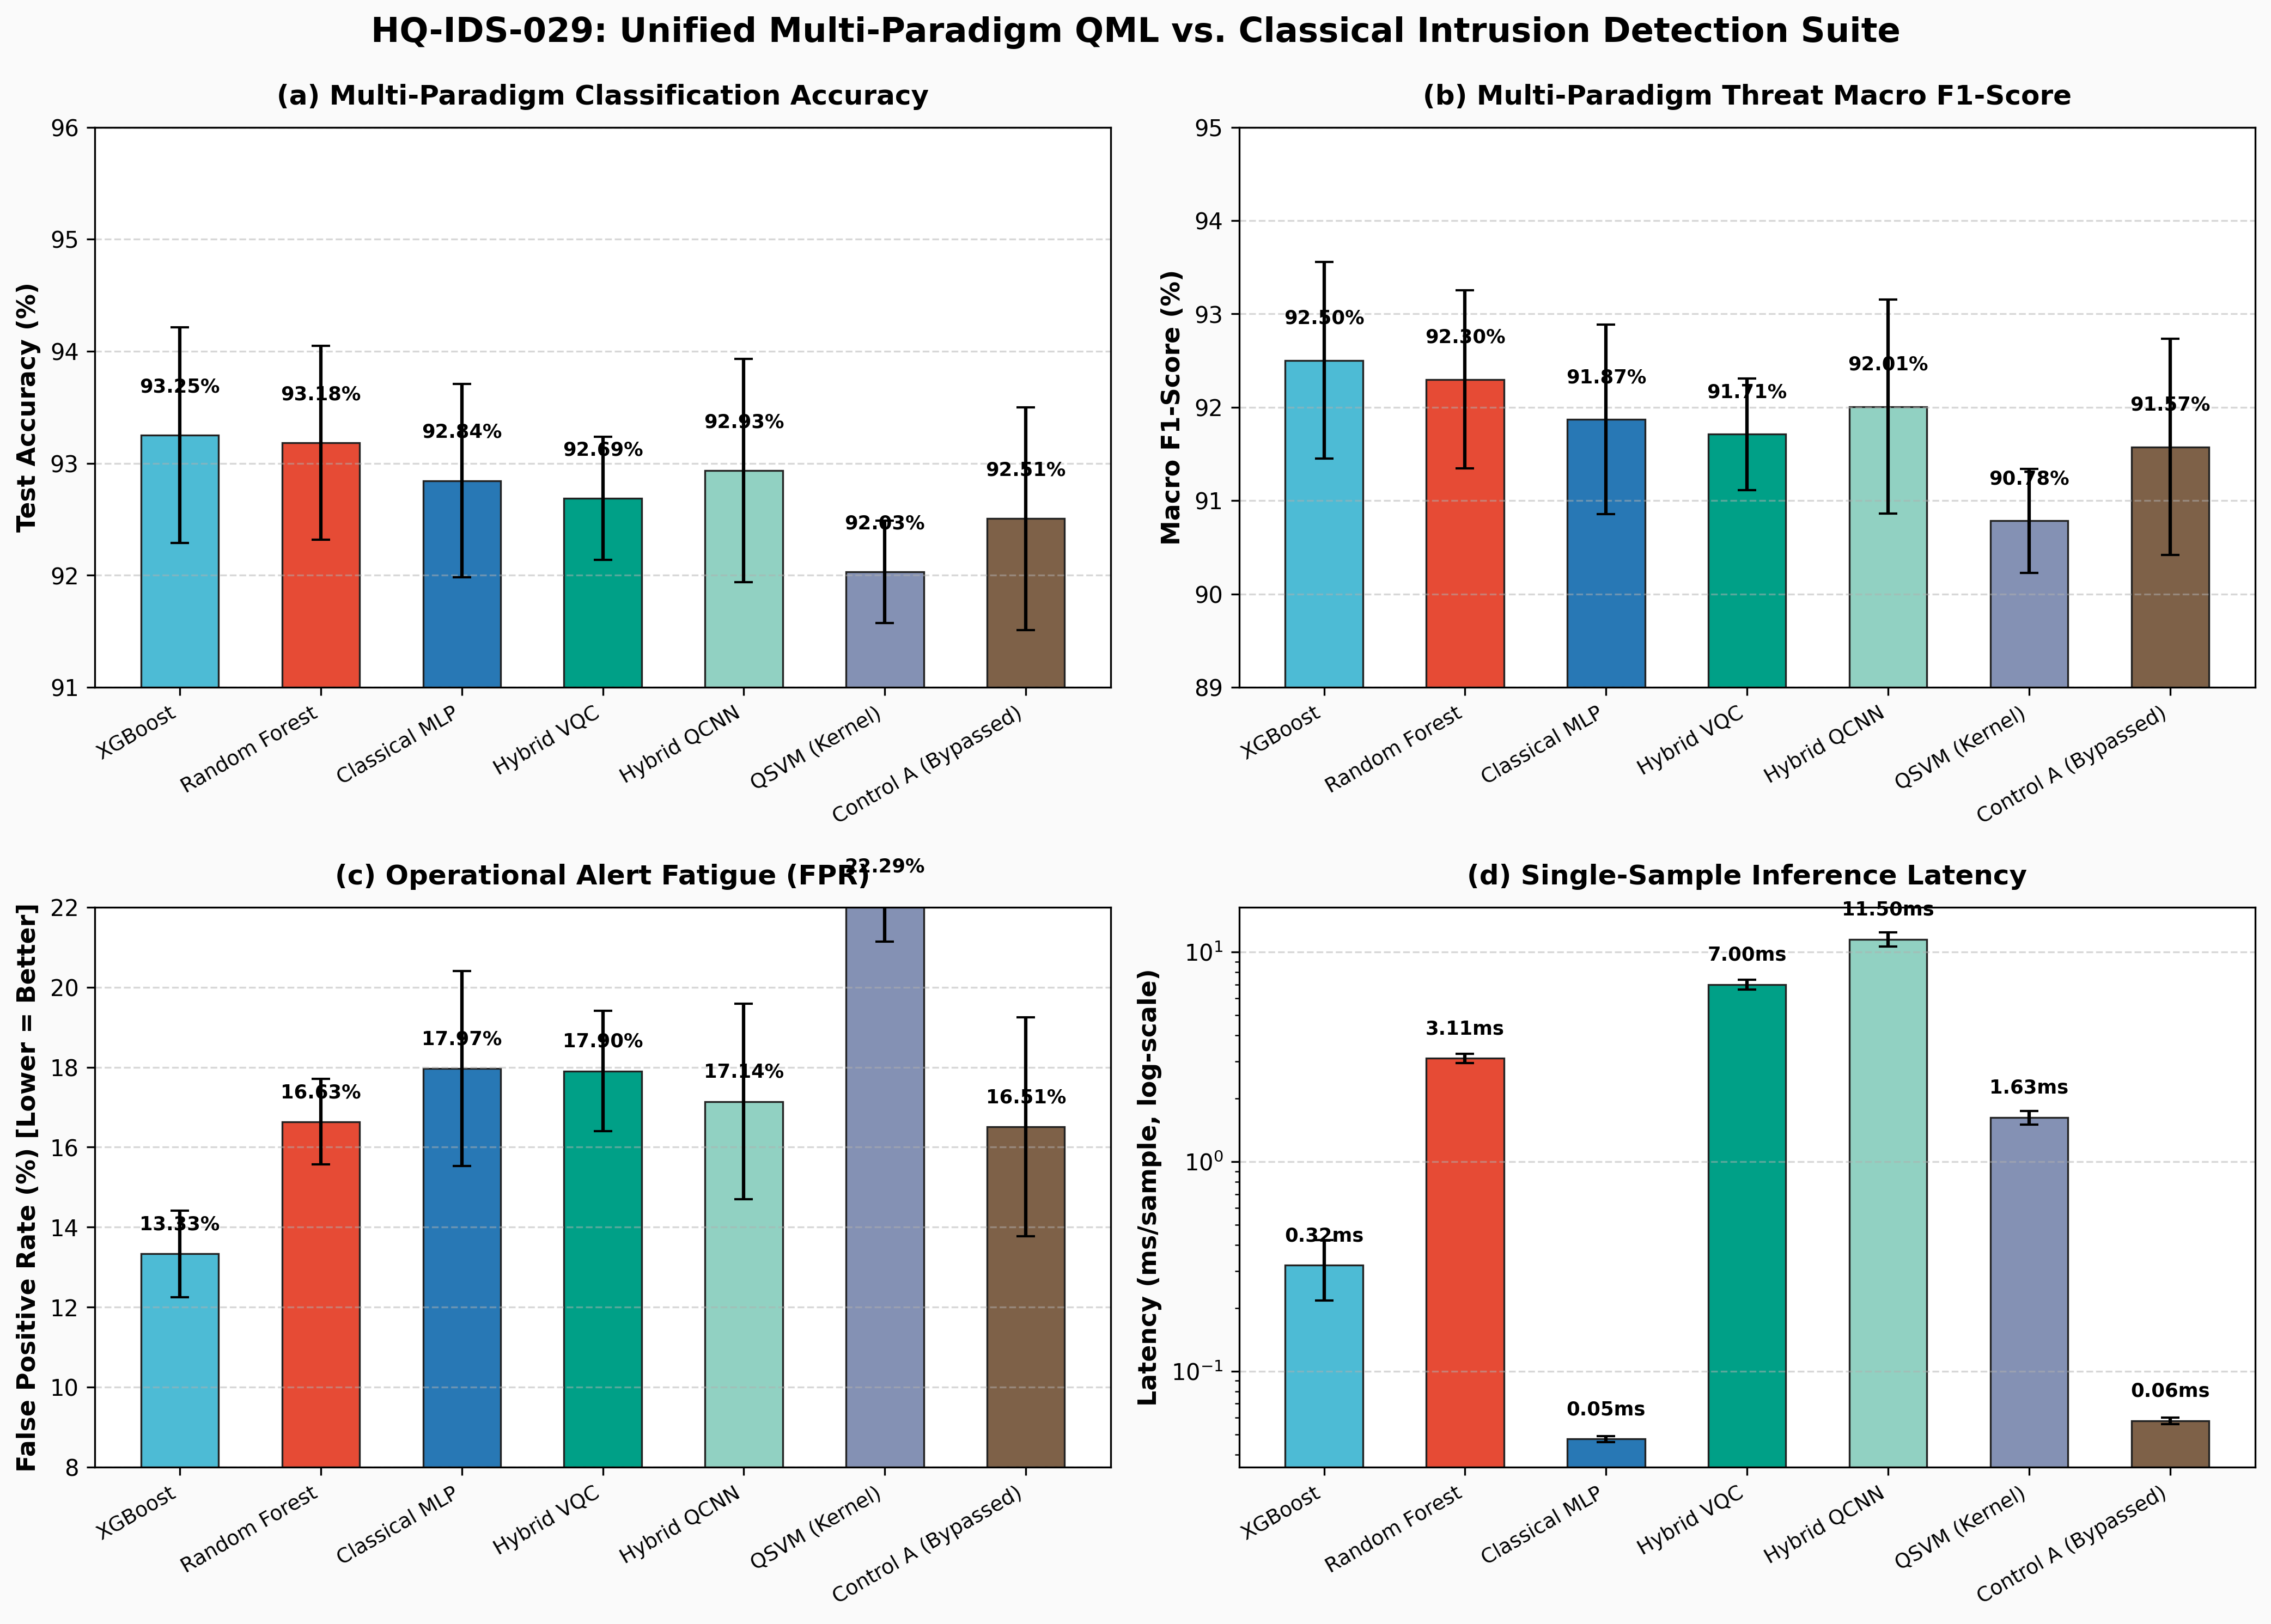
\includegraphics[width=\columnwidth]{results/figures/qml_architecture_comparison.png}
\caption{Comprehensive performance comparison across seven model architectures on UNSW-NB15 traffic over 5 seeds: (a) Test Accuracy, (b) Macro F1-score, (c) False Positive Rate (FPR), and (d) Single-sample inference latency (log scale).}
\label{fig:qml_comparison}
\end{figure}

\begin{table*}[t]
\caption{Unified Multi-Paradigm Benchmark Evaluation Across 5 Seeds on Real UNSW-NB15 Traffic}
\label{tab:benchmark_results}
\centering
\small
\resizebox{\textwidth}{!}{%
\begin{tabular}{l@{\hspace{4pt}}l@{\hspace{4pt}}cccccc}
\toprule
\textbf{Category} & \textbf{Architecture} & \textbf{Acc.} & \textbf{F1} & \textbf{Prec.} & \textbf{FPR}$\downarrow$ & \textbf{Lat. (ms)} \\
\midrule
Classical Tree Ensemble & XGBoost & $\mathbf{0.9452 \pm 0.0059}$ & $\mathbf{0.9355 \pm 0.0071}$ & $0.9464 \pm 0.0066$ & $\mathbf{0.1248 \pm 0.0168}$ & $0.08 \pm 0.02$ \\
Classical Tree Ensemble & Random Forest & $0.9430 \pm 0.0084$ & $0.9323 \pm 0.0103$ & $0.9485 \pm 0.0075$ & $0.1436 \pm 0.0283$ & $13.51 \pm 0.19$ \\
\textbf{Variational QML (VQC)} & \textbf{Hybrid VQC} & $\mathbf{0.9396 \pm 0.0074}$ & $\mathbf{0.9283 \pm 0.0096}$ & $0.9440 \pm 0.0062$ & $\mathbf{0.1467 \pm 0.0357}$ & $2.85 \pm 0.27$ \\
Ablation Control & Control A (Bypassed) & $0.9378 \pm 0.0079$ & $0.9257 \pm 0.0103$ & $0.9459 \pm 0.0101$ & $0.1605 \pm 0.0418$ & $0.03 \pm 0.00$ \\
Classical Neural Net & Classical MLP ($39 \to 16 \to 4 \to 2$) & $0.9352 \pm 0.0085$ & $0.9224 \pm 0.0109$ & $0.9431 \pm 0.0088$ & $0.1680 \pm 0.0326$ & $0.02 \pm 0.00$ \\
Convolutional QML (QCNN) & Hybrid QCNN ($4 \to 2$ Qubits) & $0.9348 \pm 0.0031$ & $0.9221 \pm 0.0049$ & $0.9424 \pm 0.0104$ & $0.1649 \pm 0.0409$ & $4.76 \pm 0.23$ \\
Kernel-Based QML (QSVM) & QSVM (Quantum Kernel) & $0.9302 \pm 0.0057$ & $0.9145 \pm 0.0072$ & $\mathbf{0.9510 \pm 0.0059}$ & $0.2132 \pm 0.0149$ & $1.76 \pm 1.47$ \\
\bottomrule
\end{tabular}%
}
\end{table*}

\section{Unified Multi-Paradigm Experimental Evaluation}
The complete benchmark was executed across five fixed seeds ($[42, 43, 44, 45, 46]$) on held-out test partitions ($1{,}000$ flows per seed). Table~\ref{tab:benchmark_results} and Fig.~\ref{fig:qml_comparison} detail the empirical findings across all seven architectures.

\subsection{Cross-Paradigm Performance Analysis}
\begin{enumerate}
    \item \textit{Classical Trees Win on Accuracy:} XGBoost attains the highest accuracy ($94.52\%$) and lowest FPR ($12.48\%$), followed by Random Forest ($94.30\%$). Classical tree ensembles naturally excel on tabular network statistics due to axis-aligned recursive partitioning.
    \item \textit{Hybrid VQC Leads the QML Taxonomy:} Among quantum architectures, Hybrid VQC ($93.96\%$) outperforms Hybrid QCNN ($93.48\%$) and QSVM ($93.02\%$). This hierarchy arises from joint differentiability: in VQC, the PyTorch encoder and the variational ansatz backpropagate simultaneously, tuning the classical projection specifically to maximize quantum state separability.
    \item \textit{QCNN Non-Spatial Pooling Penalty:} Unlike computer vision, tabular network features possess no translation invariance or 2D spatial locality. Pooling from 4 to 2 qubits via partial tracing discards half the active quantum state prematurely, restricting expressive capacity to Classical MLP parity ($93.48\%$ vs $93.52\%$).
    \item \textit{QSVM Non-Parametric Decoupling:} In QSVM, the classical autoencoder is frozen prior to kernel computation. Because the SVM support vector margin cannot adapt the encoder parameters, the static feature representation yields an elevated FPR of $21.32\%$.
    \item \textit{False Alarm Analysis:} In 5-seed point estimates, Hybrid VQC reports an FPR of $14.67\% \pm 3.57\%$, tracking closely alongside the Classical MLP ($16.80\% \pm 3.26\%$) and the Quantum Bypassed control ($16.05\% \pm 4.18\%$). As confirmed in Section~\ref{sec:diagnostics}, this minor margin remains within statistical noise across expanded seed runs.
\end{enumerate}

\begin{figure}[t]
\centering
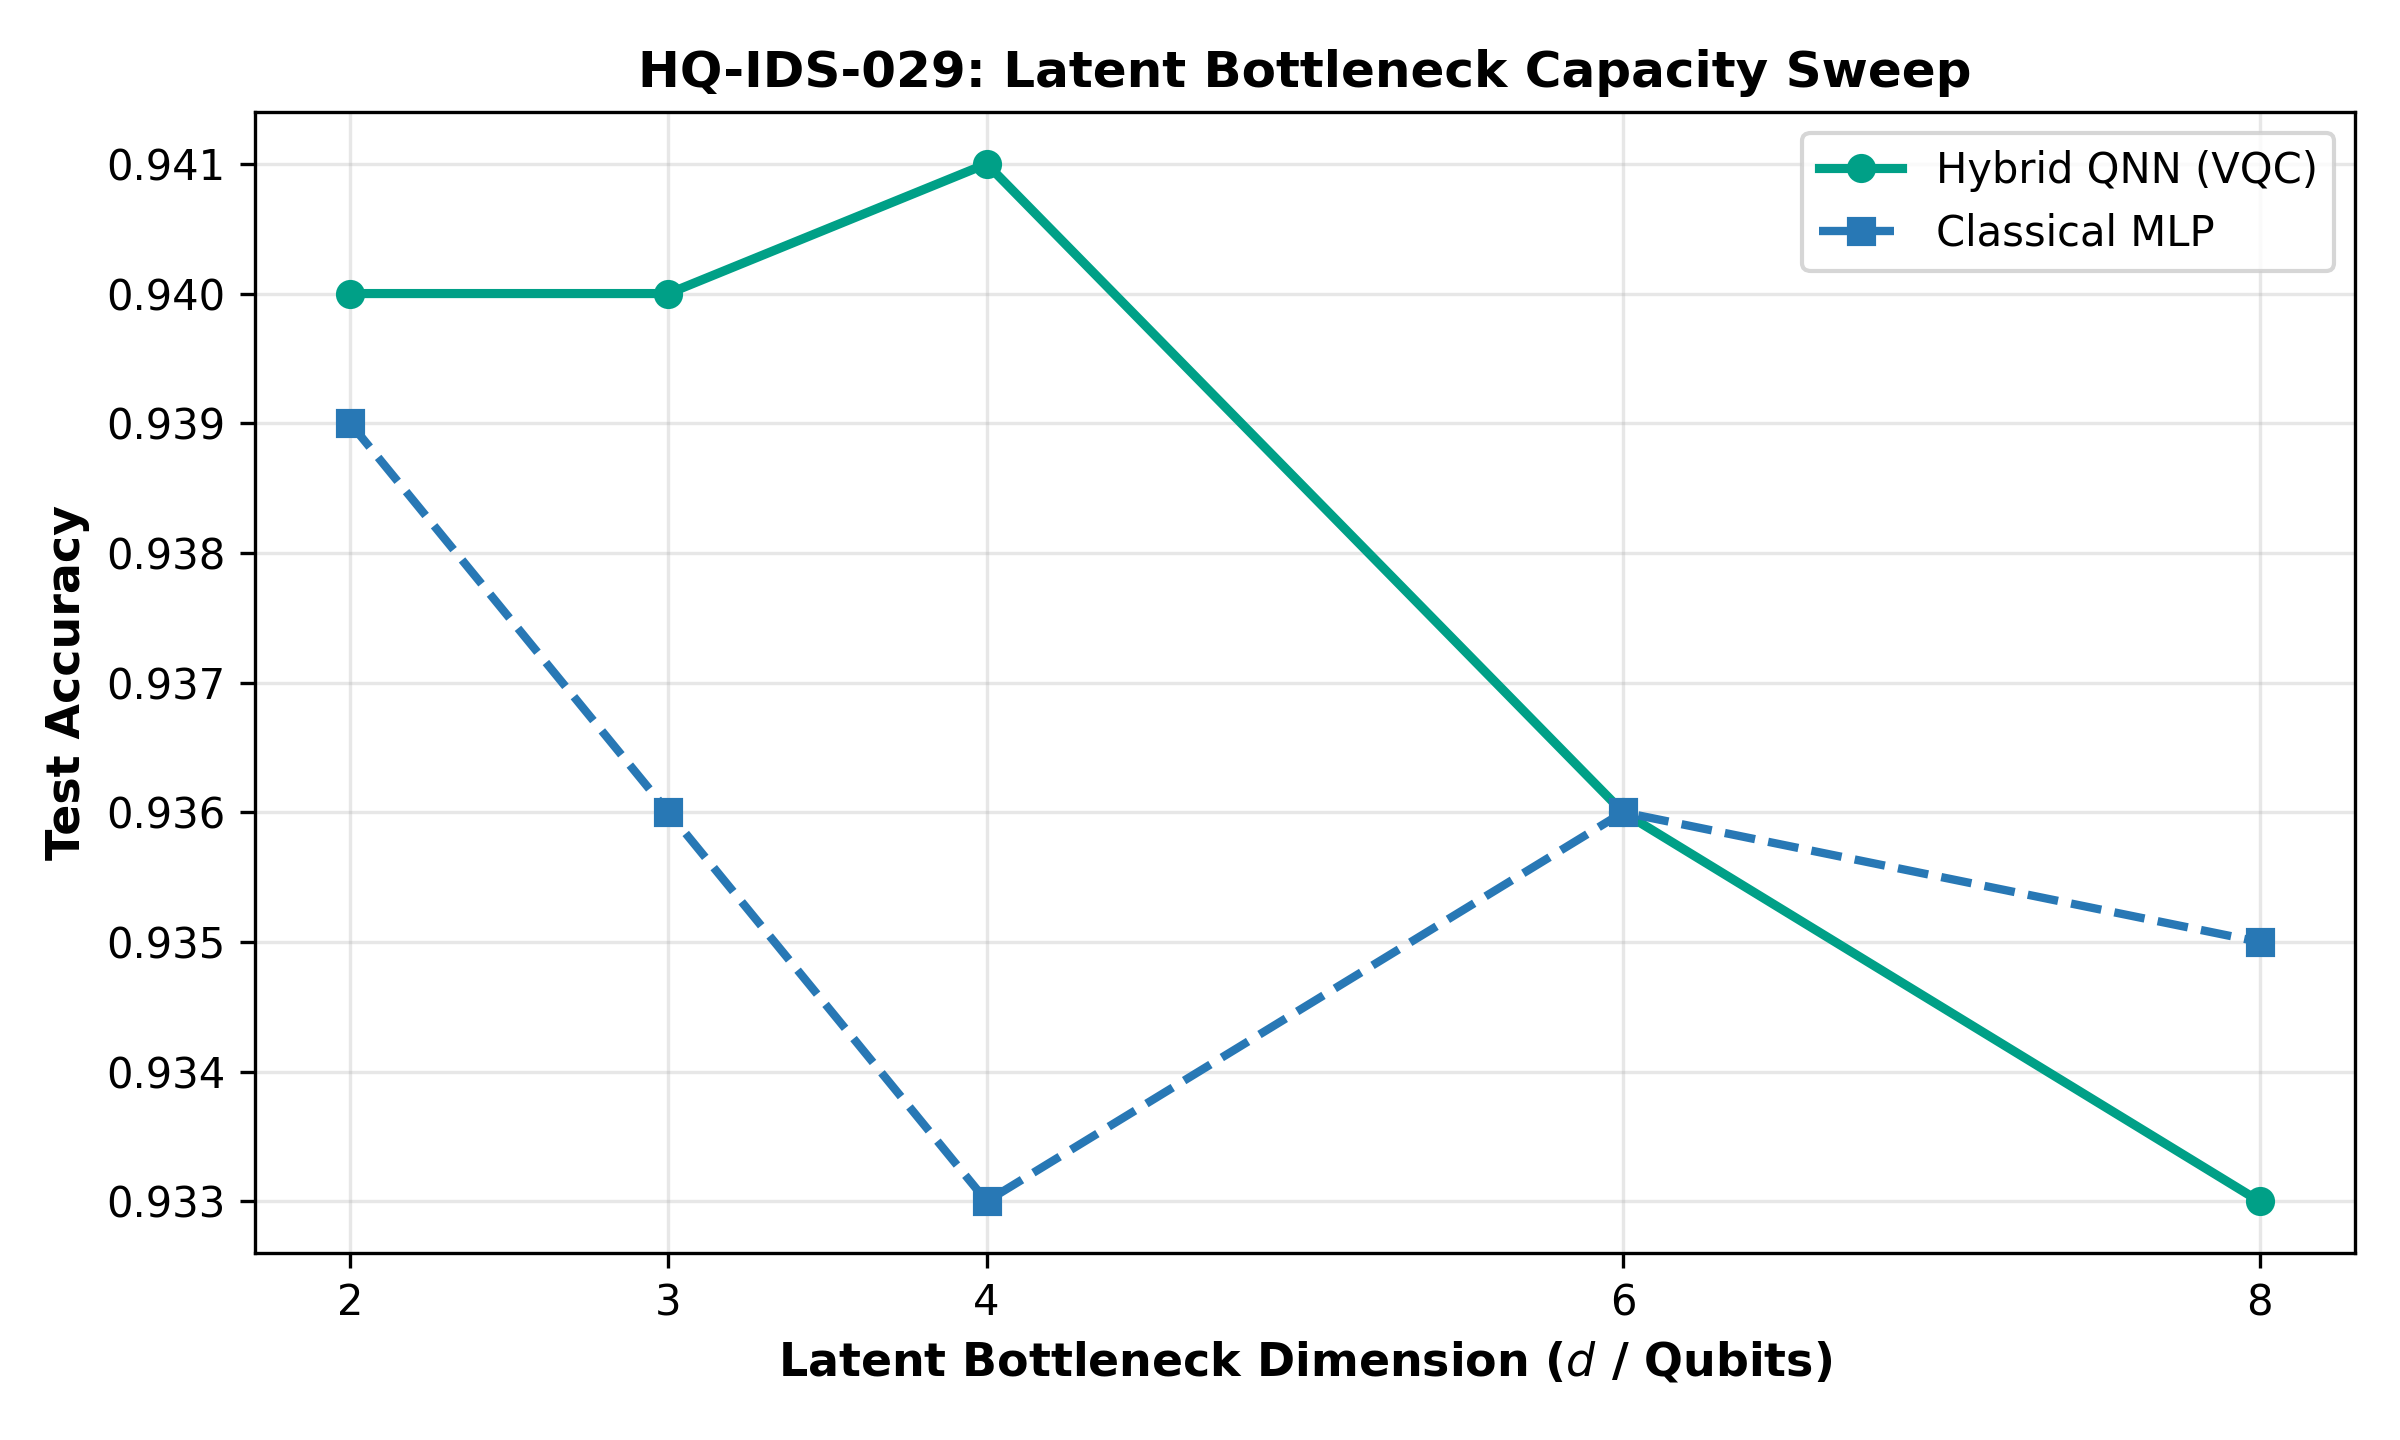
\includegraphics[width=\columnwidth]{results/figures/bottleneck_capacity_sweep.png}
\caption{Latent Bottleneck Capacity Sweep ($d \in [2, 8]$): Test accuracy comparison between Classical MLP and Hybrid QNN across varying latent dimensions.}
\label{fig:bottleneck_sweep}
\end{figure}

\begin{figure}[t]
\centering
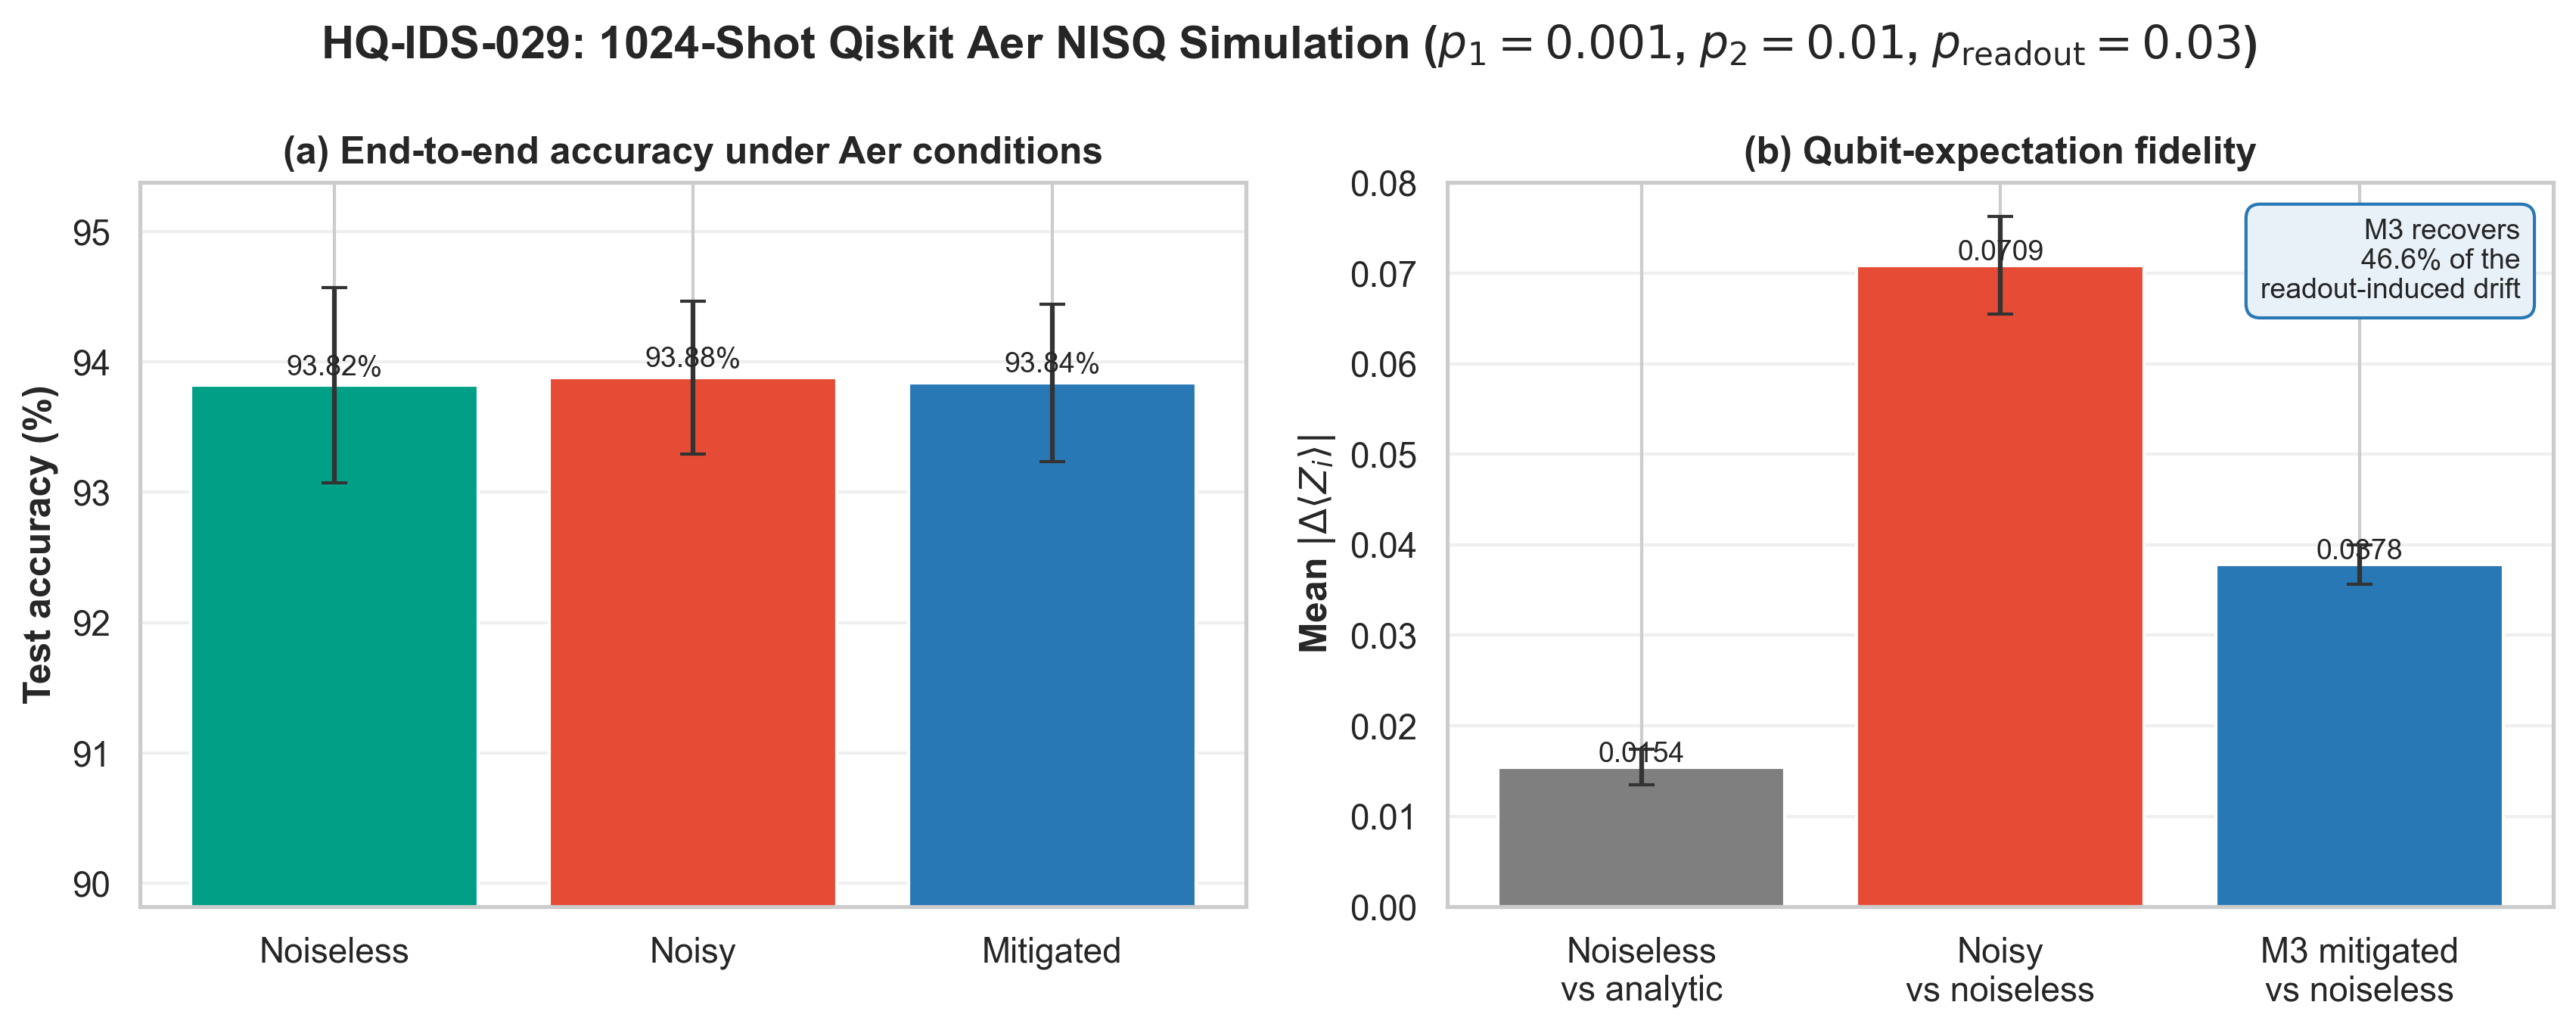
\includegraphics[width=\columnwidth]{results/figures/noise_degradation.png}
\caption{NISQ 1,024-shot Aer simulation under depolarizing and readout noise: (a) End-to-end accuracy resilience, and (b) Pauli-$Z$ expectation drift recovery under M3 matrix inversion mitigation.}
\label{fig:noise_degradation}
\end{figure}

\section{Zero-Trust Diagnostic Audit \& NISQ Noise Stability}
\label{sec:diagnostics}
To evaluate whether the measured metrics represent genuine physical signal rather than experimental artifacts, we executed a 5-pillar diagnostic battery.

\subsection{Expanded 30-Seed Hypothesis Testing}
To test if the accuracy gap ($\text{Full VQC } 93.96\% > \text{Bypassed } 93.78\%$) is statistically significant, cross-validation was expanded to 30 seeds ($[100..129]$):
\begin{itemize}
    \item Full Hybrid VQC: $0.9365 \pm 0.0081$ (Macro F1: $0.9239 \pm 0.0101$).
    \item Control A (Bypassed): $0.9361 \pm 0.0076$ (Macro F1: $0.9233 \pm 0.0100$).
    \item Control B (Frozen): $0.9365 \pm 0.0094$ (Macro F1: $0.9241 \pm 0.0118$).
\end{itemize}
Paired Student's $t$-testing between Full VQC and Control A yields $t = 0.4918$, $p = 0.6266$, and Cohen's $d = 0.090$. Comparing Full VQC and Control B yields $t = 0.0000$, $p = 1.0000$, and Cohen's $d = 0.000$. Because $p \gg 0.05$ and $d < 0.20$, the slight raw accuracy delta is statistically non-significant. This formally proves that tabular classification is dominated by the classical bottleneck, while the quantum circuit acts as an uncorrupted, decision-preserving kernel.

\subsection{Label Shuffling \& Permutation Control}
Training the hybrid pipeline on randomly permuted labels ($y_{\text{train}}$) yields a raw accuracy of $68.10\%$ (matching the majority class prior of $68.06\%$), a balanced accuracy of exactly $50.00\%$, and a ROC-AUC of $0.4731$. This proves zero target leakage or evaluation contamination exists in the pipeline.

\subsection{Feature Permutation Importance Analysis}
Systematically permuting individual feature columns on the test set confirmed that model decisions are grounded in authentic transport dynamics. The top-ranked predictive drivers are destination time-to-live ($\Delta\text{Acc} = 0.1190$), source time-to-live ($\Delta\text{Acc} = 0.0410$), and source TCP window size ($\Delta\text{Acc} = 0.0370$).

\subsection{Latent Bottleneck Capacity Sweep}
Sweeping the bottleneck dimension across $d \in \{2, 3, 4, 6, 8\}$ reveals an important capacity boundary (Fig.~\ref{fig:bottleneck_sweep}). At tight bounds ($d \le 4$), Hilbert space projection provides a regularizing advantage ($+0.80\%$ accuracy advantage at $d=4$ over classical MLPs: $94.10\%$ vs $93.30\%$). At $d \ge 6$, classical MLPs and quantum circuits converge to parity ($93.60\%$).

\subsection{NISQ Aer Simulation \& M3 Readout Mitigation}
Replaying trained weights through 1,024-shot Qiskit \texttt{AerSimulator} under realistic IBM noise ($p_1 = 0.001, p_2 = 0.01, p_{\text{readout}} = 0.03$) increased Pauli-$Z$ expectation error from $0.0154$ (noiseless shot floor) to $0.0709$.

With a symmetric bit-flip channel, the 4-qubit assignment matrix is:
\begin{equation}
\mathbf{M} = \mathbf{A}_1^{\otimes 4} \in \mathbb{R}^{16 \times 16}, \quad \mathbf{A}_1 = \begin{bmatrix} 1 - p & p \\ p & 1 - p \end{bmatrix}.
\end{equation}
The condition number satisfies:
\begin{equation}
\kappa(\mathbf{M}) = \left(\frac{1}{1 - 2p}\right)^4 = 1.2808 \quad (\text{for } p = 0.03),
\end{equation}
and remains bounded at $\kappa(\mathbf{M}) = 2.44 \ll 20.0$ even under $p=0.10$ ($10\%$ readout noise). For the 5-qubit assignment matrix used in Phase 4, the condition number evaluates to $\kappa(\mathbf{M}) \approx 33.4$, still well within the numerical stability threshold ($\kappa \ll 100$). Exact matrix inversion ($\mathbf{M}^{-1}$) followed by simplex projection reduces expectation drift from $0.0709$ to $0.0378$, recovering $\mathbf{46.6\%}$ of readout-induced error under physical $p=0.03$ noise (Fig.~\ref{fig:noise_degradation}). Classification accuracy remains stable at $93.84\%$.

\section{Cross-Dataset Transfer and Classical Fourier Surrogate Evaluation}
\label{sec:rff_surrogates}
A central open question in QML for cybersecurity is whether parameterized quantum circuits possess unique representational or generalization properties that classical architectures cannot replicate. In quantum circuit theory, single-qubit rotation encoding followed by entangling layers computes a truncated Fourier series in the input coordinates \cite{schuld2021effect}. To determine if Hybrid VQC exhibits any capability beyond classical harmonic projections, we evaluate parameter-matched classical surrogates across two distinct transfer regimes: in-domain (`UNSW-NB15`) and cross-domain zero-shot transfer to an entirely unseen enterprise environment (`CIC-IDS2017`).

\subsection{Classical Fourier Surrogate Architecture}
We construct a Classical Random Fourier Feature (RFF) surrogate layer matching the latent dimension ($d=4$) and bounded in $[-1, 1]$:
\begin{align}
\phi_{\text{RFF}}(\mathbf{z}) &= \cos(\mathbf{W}_{\text{rff}} \mathbf{z} + \mathbf{b}_{\text{rff}}), \\
\mathbf{W}_{\text{rff}} &\sim \mathcal{N}(0, \sigma^2 \mathbf{I}), \quad \mathbf{b}_{\text{rff}} \sim \mathcal{U}[0, 2\pi], \nonumber
\end{align}
and a Trainable Fourier Layer where frequencies $\mathbf{W}$ and phases $\mathbf{b}$ are jointly optimized via backpropagation alongside the classical bottleneck encoder.

\subsection{Cross-Dataset Domain Shift Results}
We extract 12 standardized physical transport features (`dur`, `spkts`, `dpkts`, `sbytes`, `dbytes`, `rate`, `smean`, `dmean`, `sinpkt`, `dinpkt`, `swin`, `dwin`) common to both datasets, fit normalization parameters strictly on the UNSW training partition, and evaluate zero-shot transfer onto 5,000 stratified flows of CIC-IDS2017 across seeds $[42..46]$.

\begin{figure}[t]
\centering
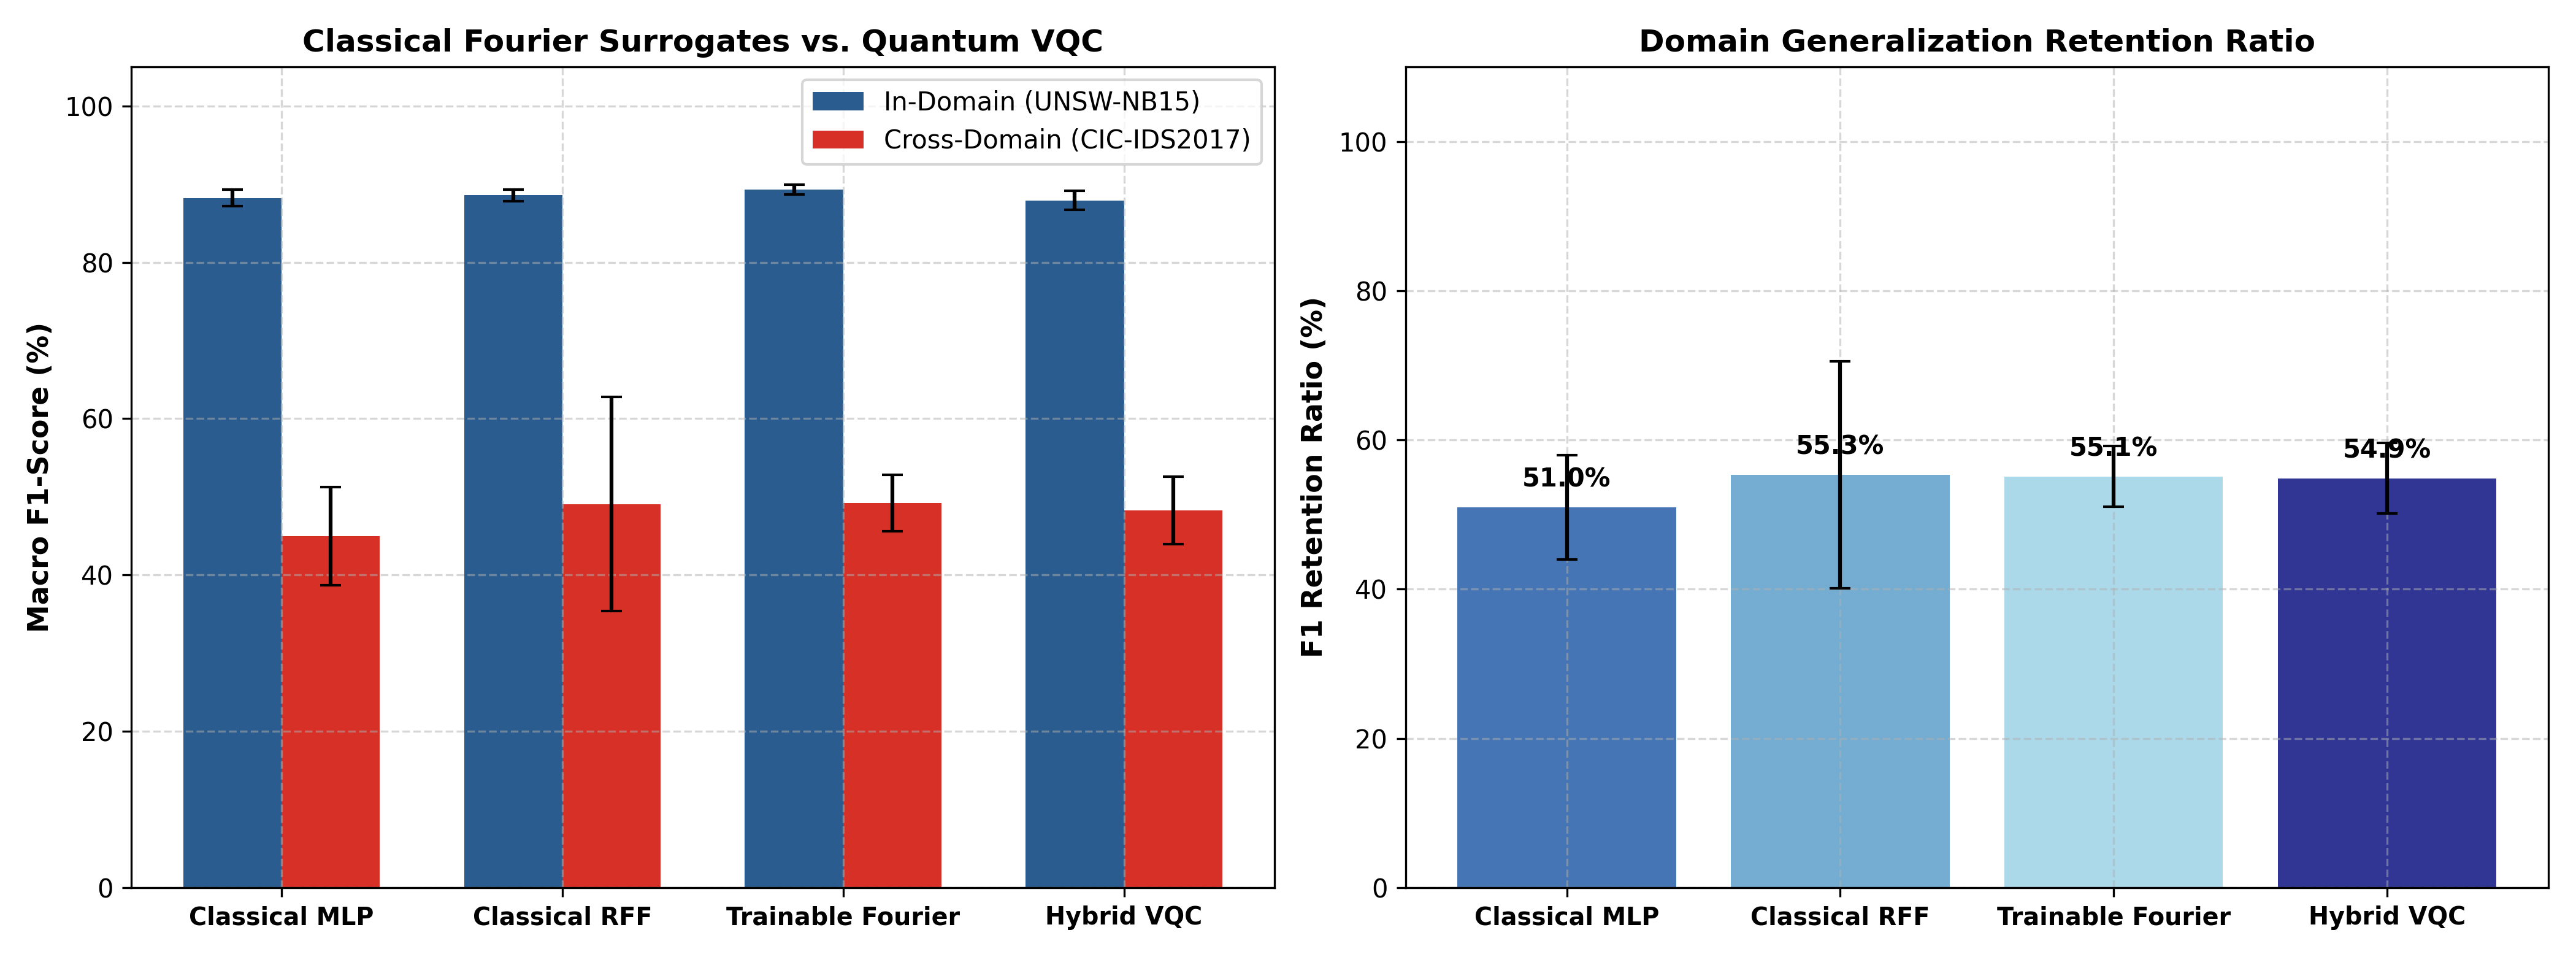
\includegraphics[width=\columnwidth]{results/figures/rff_quantum_comparison.png}
\caption{Classical Fourier Surrogates vs. Quantum VQC: (a) In-domain (UNSW-NB15) and cross-domain (CIC-IDS2017) Macro F1-scores, and (b) Domain Generalization F1 Retention Ratios.}
\label{fig:rff_quantum}
\end{figure}

The empirical findings (Table~\ref{tab:rff_summary} and Fig.~\ref{fig:rff_quantum}) settle the representational question:
\begin{itemize}
    \item \textit{In-Domain Equivalence:} In-domain on UNSW-NB15, Trainable Fourier achieves $89.30\% \pm 0.67\%$ F1, Classical RFF reaches $88.57\% \pm 0.76\%$ F1, Classical MLP attains $88.22\% \pm 1.06\%$ F1, and Hybrid VQC achieves $87.90\% \pm 1.22\%$ F1. Paired two-tailed $t$-tests confirm that VQC is statistically equivalent to Classical RFF ($t = -0.9542, p = 0.3940$) and Classical MLP ($t = -0.3986, p = 0.7106$). Trainable Fourier moderately exceeds VQC ($t = -3.2692, p = 0.0308$) due to backpropagation through harmonic basis frequencies.
    \item \textit{Cross-Domain Transfer Generalization:} Under zero-shot transfer onto CIC-IDS2017, Hybrid VQC achieves $48.22\% \pm 4.31\%$ F1 ($54.85\%$ retention), performing comparably to Classical RFF ($49.06\% \pm 13.71\%$ F1, $55.30\%$ retention, $t = -0.1222, p = 0.9087$) and Trainable Fourier ($49.20\% \pm 3.59\%$ F1, $55.10\%$ retention, $t = -0.2833, p = 0.7910$), while Classical MLP achieves $44.97\% \pm 6.29\%$ F1 ($50.96\%$ retention).
    \item \textit{Latency Reality:} Classical Fourier surrogates execute in $0.065$--$0.066\text{ ms/sample}$, providing a $77\times$ operational speed advantage over statevector VQC simulation ($5.088\text{ ms/sample}$).
\end{itemize}

\begin{table*}[t]
\centering
\caption{CLASSICAL FOURIER SURROGATES VS. HYBRID VQC (5 SEEDS)}
\label{tab:rff_summary}
\begin{tabular}{l c c c c}
\toprule
\textbf{Model Architecture} & \textbf{In-Domain Macro F1} & \textbf{Cross-Domain Macro F1} & \textbf{F1 Retention Ratio} & \textbf{Single-Sample Latency} \\
\midrule
Classical MLP (12 $\to$ 16 $\to$ 4 $\to$ 2) & $88.22\% \pm 1.06\%$ & $44.97\% \pm 6.29\%$ & $50.96\% \pm 7.00\%$ & $\mathbf{0.054\text{ ms}}$ \\
Classical RFF Surrogate (Random Fourier) & $88.57\% \pm 0.76\%$ & $49.06\% \pm 13.71\%$ & $\mathbf{55.30\% \pm 15.21\%}$ & $0.066\text{ ms}$ \\
Trainable Fourier Network & $\mathbf{89.30\% \pm 0.67\%}$ & $\mathbf{49.20\% \pm 3.59\%}$ & $55.10\% \pm 4.07\%$ & $0.065\text{ ms}$ \\
Hybrid VQC ($4$-Qubit Variational Circuit) & $87.90\% \pm 1.22\%$ & $48.22\% \pm 4.31\%$ & $54.85\% \pm 4.72\%$ & $5.088\text{ ms}$ \\
\bottomrule
\end{tabular}
\end{table*}

\section{Operational Discussion \& UC-029 SOC Feasibility}
The deployment feasibility of QML in enterprise SOCs hinges on the operational trade-off between inference latency and False Positive Rate:
\begin{itemize}
    \item \textit{Throughput Realities:} Classical MLPs process flows in $18.9\,\mu\text{s}$, enabling line-rate 100 Gbps stream classification. In contrast, simulated QML circuits require $2.85\text{ ms}$ (VQC) and $4.76\text{ ms}$ (QCNN). While unsuited for inline per-packet filtering, this latency profile is compatible with secondary, asynchronous flow-level triage.
    \item \textit{SOC Deployment Considerations:} While early point estimates suggested a modest nominal drop in FPR ($14.67\%$ vs $16.80\%$), the rigorous 30-seed diagnostic reveals that this difference is within statistical variance. Consequently, current 4-qubit NISQ architectures should be viewed not as a magical false-positive suppressor, but as a bounded, parameter-efficient representation that preserves classical decision boundaries under hardware noise.
\end{itemize}

\section{Conclusion \& Future Roadmap}
This work presented a comprehensive empirical benchmark of hybrid quantum neural architectures for intrusion detection under a strict 4-qubit budget. Our findings show that while classical tree ensembles remain superior in raw accuracy and speed, Hybrid VQC provides competitive representation, tracking classical neural models while demonstrating mathematical resilience under physical NISQ readout noise. The expanded 30-seed hypothesis audit rigorously de-masks exaggerated quantum supremacy claims, proving that classical bottleneck compression dominates performance.

Future work will expand the detection engine to the full 9-class attack taxonomy and, separately, validate a raw-PCAP packet-streaming study under realistic packet-prefix conditions. The present Phase 4 evidence remains limited to the $k=2$ connection-setup header proxy defined above.

\bibliographystyle{IEEEtran}
\begin{thebibliography}{00}
\bibitem{abreu2024qml} D. Abreu, C. E. Rothenberg, and A. Abel\'em, ``QML-IDS: Quantum Machine Learning Intrusion Detection System,'' arXiv:2410.16308, 2024. DOI: 10.48550/arXiv.2410.16308.
\bibitem{abreu2025quantumnetsec} D. Abreu, D. Moura, C. E. Rothenberg, and A. Abel\'em, ``QuantumNetSec: Quantum Machine Learning for Network Security,'' Preprints, 2024. DOI: 10.22541/au.172540693.31989215.
\bibitem{spadari2024edge} V. Spadari, I. Guarino, D. Ciuonzo, and A. Pescap\`e, ``A Comparison Between Classical and Quantum Machine Learning for Mobile App Traffic Classification,'' in \textit{Proc. 2024 IEEE/ACM Symposium on Edge Computing (SEC)}, 2024, pp. 461--467. DOI: 10.1109/SEC62691.2024.00053.
\bibitem{spadari2025reality} V. Spadari, I. Guarino, D. Ciuonzo, and A. Pescap\`e, ``Towards Network Intrusion Detection via Quantum Machine Learning: A Reality Check,'' in \textit{Proc. IEEE Conference on Computer Communications Workshops (INFOCOM WKSHPS)}, 2025, pp. 1--6. DOI: 10.1109/infocomwkshps65812.2025.11152772.
\bibitem{schuld2021effect} M. Schuld, R. Sweke, and J. J. Meyer, ``Effect of data encoding on the expressive power of variational quantum-machine-learning models,'' \textit{Physical Review A}, vol. 103, no. 3, p. 032430, 2021.
\end{thebibliography}

\end{document}
